\documentclass{article}
\usepackage[utf8]{inputenc}
\usepackage{setspace} 
\usepackage{enumitem}
\usepackage{geometry}
 \geometry{
 a4paper,
 left=30mm,
 right=30mm,
 top=30mm,
 }

\title{\textbf{Urban Sound Classification with Support Vector Machines}}
\author{Person codes: 10783942, 10561598, 10500756, 10583734, 10472602}
\date{April 2021}


\usepackage[numbers, square, sort]{natbib}
\usepackage{graphicx}
\usepackage{amsmath}
\usepackage{url}
\newcommand{\code}{\texttt}
\usepackage[justification=centering]{caption}

\begin{document}

\maketitle

\section{Introduction}
This report describes the implementation of a classifier, which is capable of predicting different types of sound events occurring in audio excerpts. In particular, the goal is to classify common urban environment sounds such as a dog bark, a jackhammer sound or a car horn.\\
The work was divided into several parts in a modular fashion, and this report is organized as follows. Section 2 presents an overview of the dataset and shows the results of the preliminary studies of the dataset. Section 3.1 illustrates the processing of the audio excerpts, which are used to compute several features. The features are then stored inside a JSON file. Section 3.2 describes the training and validation procedure. Our classifier is implemented as a support vector machine (SVM) with 10-fold cross validation. In Section 3.3, we outline the adoption of parallelization procedures, which decrease dramatically the time needed for the feature computation, training and validation. Section 4 presents the obtained results. In section 5, we point out possible shortcomings and future improvements of our model. 


\section{Dataset overview and analysis}
The dataset used for the Homework is the \textbf{Urbansound 8k} dataset, which has been proposed in \cite{SalamonUrbanSound}. It consists of 8732 labeled sound excerpts with short duration ($\leq 4s$) of urban sounds, and is subdivided into 10 folds. Each fold contains excerpts from 10 different classes:
\begin{enumerate}[itemsep=0em]
    \item Air conditioner
    \item Car horn
    \item Children playing
    \item Dog bark
    \item Drilling
    \item Engine idling
    \item Gunshot
    \item Jackhammer
    \item Siren
    \item Street music
\end{enumerate}
As a first step, the dataset was downloaded and studied in a Python dataset analysis notebook \cite{githubRepo}. This dataset comes with a \code{.csv} metadata file, which contains exhaustive details about every audio excerpt. The \code{.csv} file was imported in a suitable data structure - a Dataframe from the Pandas library \cite{pandas}. After that, the sample distributions were analyzed. The results are reported in the histograms in Figure \ref{fig:samples_histogram} and in Tables \ref{tab::samples_per_fold} - \ref{tab::samples_per_class}, which show the number of samples for each fold and for each class. What catches the eye is that the \texttt{car\_horn} and \texttt{gun\_shot} classes are the least represented ones. However, these classes present the lowest intra-class variability, meaning that less excerpts are sufficient to characterize the entire class. Therefore, it was not deemed necessary to perform data augmentation.

\begin{figure}[ht]
    \centering
    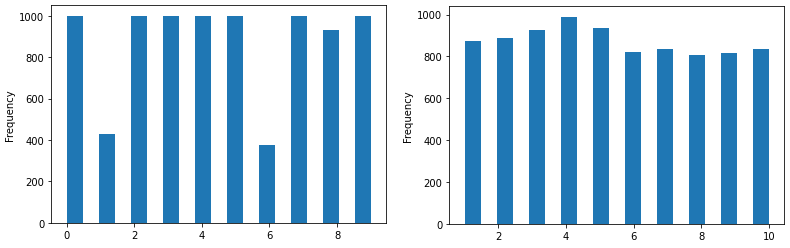
\includegraphics[scale=0.4]{img/SamplesPerClass_SamplesPerFold.png}
    \caption{Histogram of audio samples per fold (\textbf{left}) and per class (\textbf{right})}
    \label{fig:samples_histogram}
\end{figure}

\begin{table}[ht]
\centering
\begin{tabular}{|l|l|l|l|l|l|l|l|l|l|l|}
\hline
\textbf{Fold n.}          & 1   & 2   & 3   & 4   & 5   & 6   & 7   & 8   & 9   & 10  \\ \hline
\textbf{N. of samples} & 873 & 888 & 925 & 990 & 936 & 823 & 838 & 806 & 816 & 837 \\ \hline
\end{tabular}
\caption{Samples per fold}
\label{tab::samples_per_fold}
\end{table}



\begin{table}[ht]
\centering
\begin{tabular}{|l|l|}
\hline
\textbf{Class}    & \textbf{N. of samples} \\ \hline
air\_conditioner  & 1000                   \\ \hline
car\_horn         & 429                    \\ \hline
children\_playing & 1000                   \\ \hline
dog\_bark         & 1000                   \\ \hline
drilling          & 1000                   \\ \hline
engine\_idling    & 1000                   \\ \hline
gun\_shot         & 374                    \\ \hline
jackhammer        & 1000                   \\ \hline
siren             & 929                    \\ \hline
street\_music     & 1000                   \\ \hline
\end{tabular}
\caption{Samples per class}
\label{tab::samples_per_class}
\end{table}

\section{Method}
To improve code scalability, the implementation was organized into three distinct modules inside three Google Colaboratory \cite{googleColab} notebooks:
\begin{enumerate}
    \item A dataset analysis notebook\footnote{\url{https://github.com/magiwanders/CMLS_HW1/blob/master/src/0_DatasetAnalysis.ipynb}}
    \item A feature computation and feature analysis notebook\footnote{\url{https://github.com/magiwanders/CMLS_HW1/blob/master/src/1_FeatureAnalysisAndComputation.ipynb}}
    \item A support vectore machine (SVM) training and validation notebook\footnote{\url{https://github.com/magiwanders/CMLS_HW1/blob/master/src/2_TrainingSVM.ipynb}}
\end{enumerate}
The goal of the first notebook is to extract and plot the necessary metadata from the dataset, which are contained in the complementary \code{.csv} file. The second notebook computes the features upon which the model can be trained, and stores them in a JSON file. In the third notebook, a support vector machine (SVM) is trained and tested using the aforementioned features. The model is then validated.


\subsection{Feature extraction}
The feature extraction was implemented in the feature computation and analysis Python notebook. For each audio excerpt, we extracted the Mel-Frequency Cepstral Coefficients (MFCC) using the \code{librosa} audio library \cite{librosa} and the \code{pandas} data structure \cite{pandas} library. The choice of MFCCs was motivated by the fact that the samples pertain to classes which present different noisy-harmonic character. Therefore, Mel-Frequency Cepstral Coefficients seemed as the best feature that could keep track of such detailed content. 
To compute the MFCCs, the following steps were followed: the spectrogram of the audio signal was computed by calculating the magnitude of the Short-time Fourier transform (STFT). Then, Mel filters were applied to the spectrogram and the logarithm was calculated. Finally, the Discrete Cosine Transform was applied. Table \ref{tab::MFCC_parameters} shows all the parameters that were chosen for the MFCC computation.\\
After the computation of the MFCC, five feature statistics were extracted for each audio excerpt:
\begin{enumerate}[itemsep=0em]
    \item Minimum
    \item Maximum
    \item Mean
    \item Median
    \item Variance
\end{enumerate}
Each MFCC has 25 coefficients; therefore, the combination of the five statistics resulted in 125 feature parameters extracted for every audio file. As previously mentioned, all the extracted features were then exported into a JSON file, in order to make the training procedure independent from the feature extraction part.

\begin{table}[ht]
\centering
\begin{tabular}{|c|c|}
\hline
\textbf{Parameter} & \textbf{Value}        \\ \hline
Sampling Frequency & 22050 Hz              \\ \hline
Window length   & 22.3 ms               \\ \hline
Hop Size           & 50\%                  \\ \hline
Mel filters        & 40                    \\ \hline
MFCCs              & 25                    \\ \hline
Min. frequency     & 0 Hz                  \\ \hline
Max. Frequency     & 22050 Hz              \\ \hline
\end{tabular}
\caption{Feature extraction parameters}
\label{tab::MFCC_parameters}
\end{table}


\subsection{Training and validation procedure}
The training was developed in the SVM training notebook. The first step was to retrieve the Dataframe of the computed features, which had been previously stored in a JSON file named \code{extracted\_features.json}. From here, the folds were divided iteratively in order to perform cross-validation: each fold was used only once as validation set, against the remaining 9 used as training set. For every fold iteration, the validation accuracy for each class and the confusion matrices were computed. Finally, a mean of the accuracies and confusion matrices was derived, in order to provide general performance value for the chosen classifier. 
The support vector machine was implemented with a \code{'poly'} kernel and a \code{OneVsRestClassifier} from the \code{sklearn} library \cite{sklearn}. The \code{OneVsRestClassifier} enables multi-class classification by dividing the problem into binary classification tasks between a selected class and the rest of the classes.

\subsection{Remarks on performance and parallelization}
Performance optimization was a key principle for the entire code base of the homework. Whenever possible, processing was parallelized by exploiting all available processing cores of the host machine, leading up to a ten fold improvement in terms of processing time. This was implemented with the \code{p\_tqdm} library \cite{pTdqm}, a wrapper of the \code{multiprocessing} and \code{tqdm} libraries \cite{pathos}\cite{tdqm}, which also shows a progress bar for parallel computation tasks.\\
Empirical experimentation showed that the computational overhead of the parallelization process was better diluted for the parallelization of a very small number of very computationally long tasks, as opposed to a big number of relatively short tasks. This is mostly true for machines with a relatively limited number of processing cores, which is a reasonable assumption for most consumer desktops. Were the available number of cores much higher, say 32 or 64, the sheer number of concurrent threads would overweight the computation length in spreading the overhead computational cost. Therefore, it was therefore decided to split the parallelization as early as possible in the computational process, in order to obtain maximum performance. The only downside of this approach is purely aesthetic, and almost ascribable to a sub-optimal implementation of the \code{p\_tqdm} library: since in this particular case all the parallelized tasks are roughly equivalent in required computational time, the progress bar will fill very quickly towards the end of the computation after a prolonged period of apparent inactivity. Although the lack of such feedback is certainly lacking in interaction design, it was judged a minor issue.\\
The computation thread was split twice: during feature extraction and during SVM training. Feature extraction was split into a maximum of 10 threads, each corresponding to the processing of all the samples within one folder. As mentioned before, this is only computationally convenient for host machines with a limited number of processing cores (theoretically at most 10, since 10 is the number of folders). All our machines satisfied this constraint. As was hinted before, limiting the number of threads would have been counter-productive for machines with much higher core count. The SVM training was similarly split into 10 threads, each for a different step of the cross-validation procedure. A scheme of the parallelization is shown in Figure \ref{fig:parallelization_scheme}.

\begin{figure}[h]
    \centering
    
\includegraphics[scale=0.4]{img/Simplified_Scheme.png}
    \caption{Simplified scheme of the code structure, with emphasis on visualizing parallelization}
    \label{fig:parallelization_scheme}
\end{figure}

\section{Obtained results}
By looking at the confusion matrices and the resulting accuracy of every fold iteration, it can be seen that the model reached an averaged accuracy around 49.3\%. By giving a first glance at the mean confusion matrix in Figure \ref{fig:mean_confusion_matrix}, it would seem that the classes \code{car\_horn} and \code{gun\_shot} have the worst results. However, it is quite the opposite: these two classes have the highest number of correctly predicted samples (True Positives) and the lowest amount of False Positives and False Negatives. This can be seen by the fact that the rows and columns corresponding to each of these classes are quite dark. The seemingly dim color associated to the True Positives is simply due to the fact that these classes are the least represented ones inside the dataset. 
Other classes also reach a fairly good prediction accuracy. However, it can be observed that \code{engine\_idling}, \code{air\_conditioner}, \code{jackhammer} and \code{drilling} seem to have low inter-class variability and this leads to wrong separation of these classes. 

\begin{figure}[h]
    \centering
    \caption{Final Confusion Matrix}
    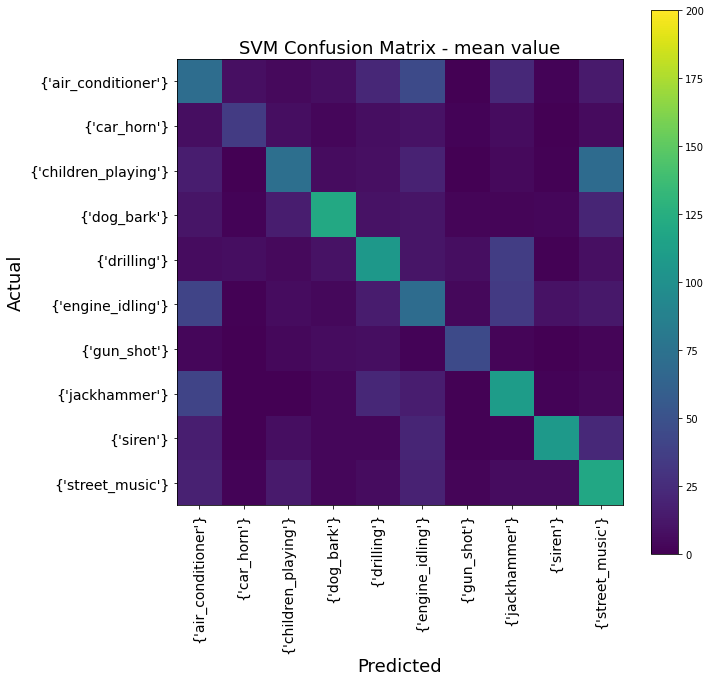
\includegraphics[scale = 0.5]{img/final_confusion_matrix.png}
    \label{fig:mean_confusion_matrix}
\end{figure}

\section{Conclusion and possible improvements}
The results of the work led us to a number of conclusions.\\
The first one is that MFCCs are maybe not best suited for the distinction between different types of noisy-like sounds.\\
Another remark is that the dataset contains both foreground and background sounds. It is reasonable to assume that background sounds makes the classification task harder, because the sound event features are less prominent in these kind of excerpts.\\
For what concerning the MFCC feature statistics, we chose to use the minimum, maximum, mean, median and variance. It is possible that the computation of second-order statistics (e.g. first derivative, second derivative) may have increased the model accuracy.\\
A last observation is directed towards our choice of adopting an SVM model. Convolutional neural networks would have probably reached a higher accuracy; however, we chose a more traditional machine learning approach to abide by the program of the course, and to put into practice the concepts shown during class. 


%Force refs to go into new page
\newpage
\bibliographystyle{unsrtnat}
\bibliography{references}
\end{document}
